\section{Proposed}
\subsection{Data Preprocessing}
\begin{figure}[tbh]
    \centering
    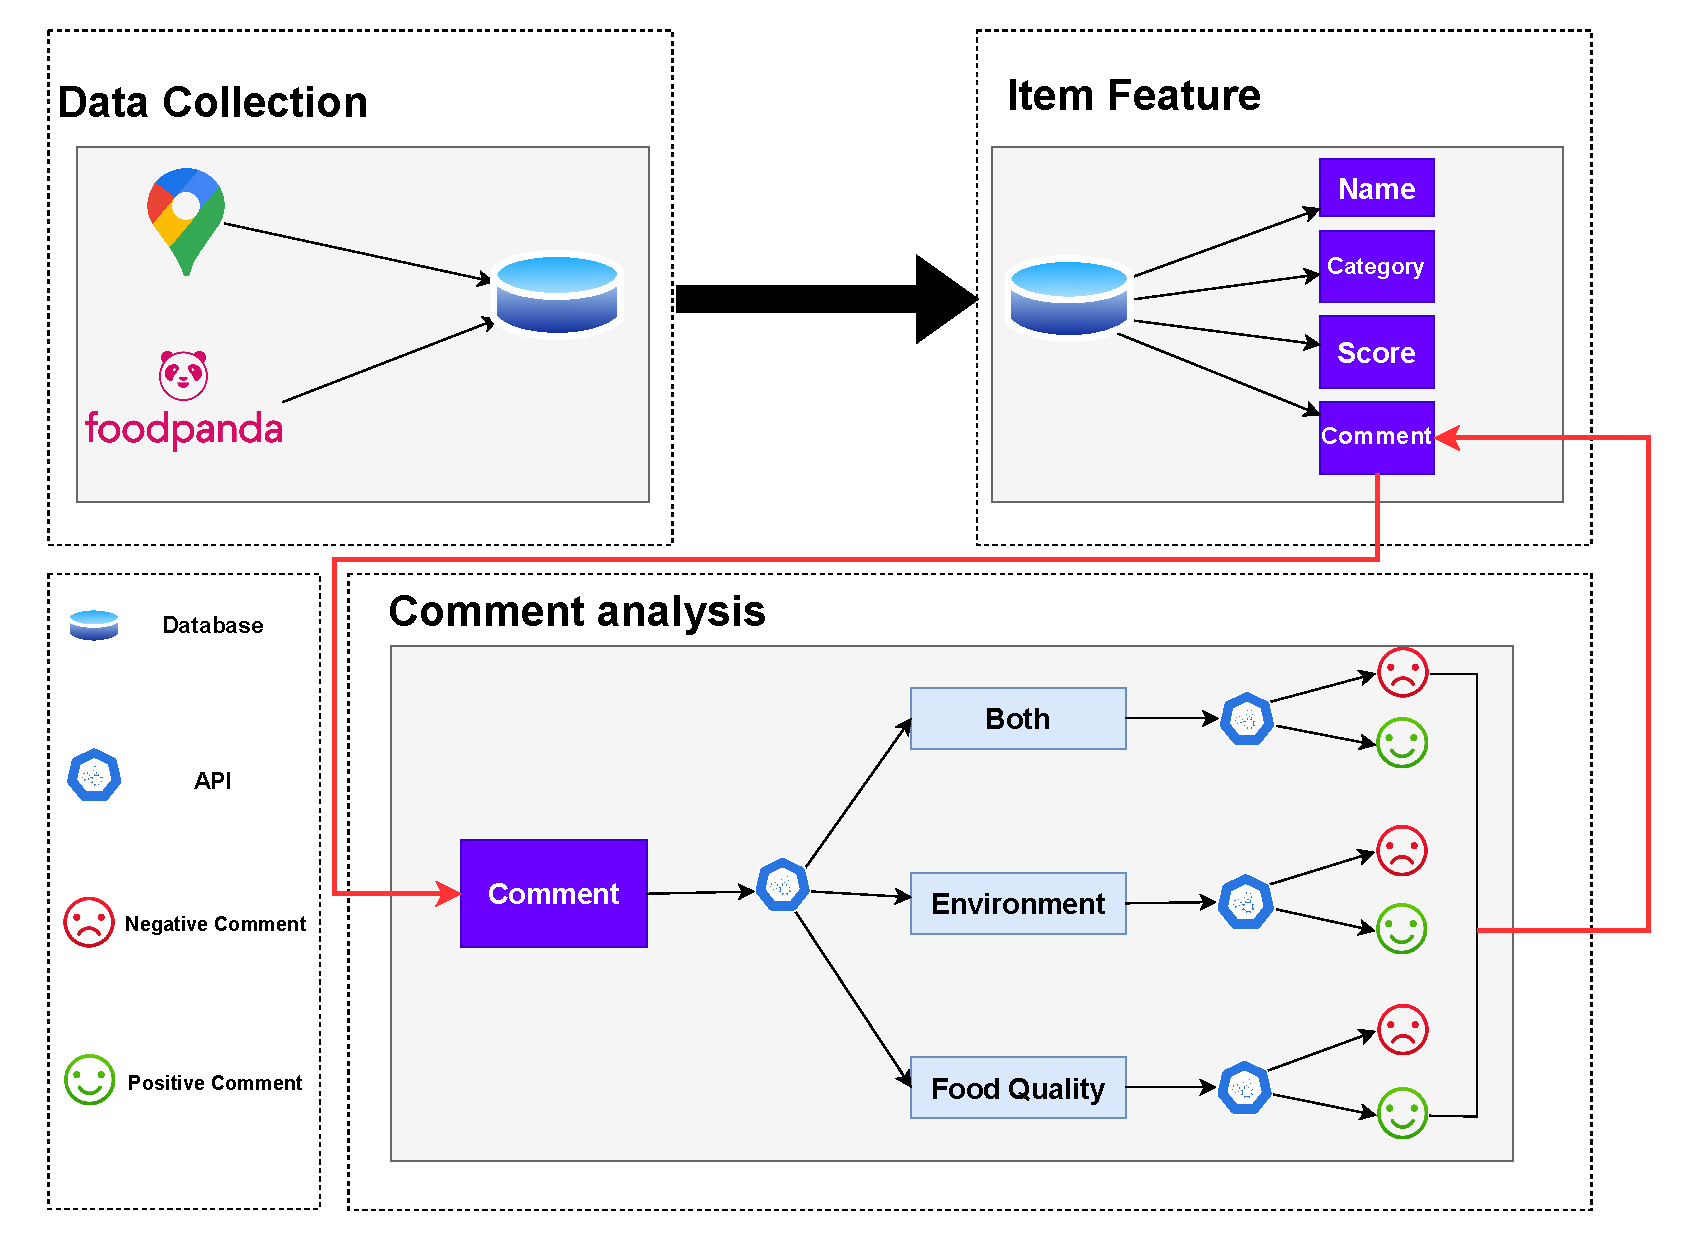
\includegraphics[width=0.5\textwidth]{img/preprocess.pdf}
    \caption{資料前處理架構圖}
    \label{fig-preprocess}
\end{figure}
本研究的資料前處理架構如\xfig{fig-preprocess}所示,利用爬蟲技術從多個平台(如 Foodpanda 和 Google Maps)獲取餐廳資料,並將資料集分為餐廳名稱、餐廳類型、評分及評論等類別。考慮到將所有評論合併可能會影響大規模語言模型(LLM)的微調效果,本研究首先採用 LLM 對評論進行分類,確定其屬於評價餐點、環境氣氛,或同時屬於這兩類中。其中對於已分類的評論,再次進行分類,以判斷其屬於正面評價還是負面評價。
\subsection{Model}
\color{blue}
本研究採用之~NIE-GCN~\cite{NIE-GCN}~內部可拆成以下步驟,第一步會先對每個餐廳節點 $i$ 做向量嵌入,得到 $d$ 維的向量 $e_i \in \mathbb{R}^d$,將每個個餐廳節點 i 的嵌入向量蒐集後可表達成下式 
\begin{equation}
    E_I^{(0)} = \{e_{i_1}^{(0)}, e_{i_2}^{(0)},\cdots,e_{i_N}^{(0)}\} \in \mathbb{R}^{N \times d},
\end{equation}
其中 $N$ 為餐廳節點的總數,$d$ 為嵌入向量之維度,上標~$0$~為第~$0$~層傳播的狀態。
得到每個餐廳節點的嵌入向量後,因使用者節點 $u$ 之鄰居必為餐廳節點,因此透過與使用者有互動之餐廳節點來推敲使用者的習性。

第二步要建構使用者節點的初始嵌入向量~$e_u^{0}$~,需透過使用者相鄰的餐廳節點 $i$ 之嵌入向量~$e_i^{0}$~建構,第~$0$~層建構方式如下式,
\begin{equation}
    e_u^{(0)} = \sigma (\sum_{i \in N_u} \frac{1}{\sqrt{\vert N_u \vert \vert N_i \vert}}e_i^{(0)}),
\end{equation}
其中 $N_u$、$N_i$ 分別為使用者節點 $u$ 和餐廳節點 $i$ 之鄰居,$\sigma(\cdot)$ 為雙曲正切函數~(tanh)。
有了 $e_u$ 和 $e_i$ 後,下一步要去計算與使用者節點 $u$ 相鄰之餐廳節點 $i$ 連線的注意力分數,來決定鄰居點的重要性,其計算方式如下式
\begin{equation}
    \rho(u, i) = Q^T\sigma(W(e_u^{(0)}||(e_i^{(0)})+b)),
\end{equation}
其中 $W \in \mathbb{R}^{2d \times d}$、$Q \in \mathbb{R}^{1 \times d}$、$b \in \mathbb{R}^{1 \times d}$,這三個都是注意力機制中的權重矩陣,$\sigma(\cdot)$ 為雙曲正切函數~(tanh),$||$ 為向量串接,若 $\rho(u, i)$ 的分數越高則代表 $u$ 和 $i$ 之間的存在更高的關聯性,最後這些注意力分數再使用 Softmax 範圍限制在 $[0,1]$ 之間,得到 $\alpha(u, i)$,並以該值作為最終使用者節點 $u$ 和餐廳節點 $i$ 之間的注意力值。
\begin{equation}
    \alpha(u, i) = \frac{\exp(\rho(u, i))}{(\sum_{j \in N_u}\exp(\rho(u, j)))^{\beta}}.
\end{equation}
\color{black}